%%%%%%%%%%%%%%%%%%%%%%%%%%%%%%%%%%%%%%%%%%%%%%%%%%%%%%%%%%%%%%%%%%%%
%% I, the copyright holder of this work, release this work into the
%% public domain. This applies worldwide. In some countries this may
%% not be legally possible; if so: I grant anyone the right to use
%% this work for any purpose, without any conditions, unless such
%% conditions are required by law.
%%%%%%%%%%%%%%%%%%%%%%%%%%%%%%%%%%%%%%%%%%%%%%%%%%%%%%%%%%%%%%%%%%%%

\documentclass{beamer}
\usetheme[faculty=phil]{fibeamer}
\usepackage[utf8]{inputenc}
\usepackage[
  main=english
]{babel}
%% These macros specify information about the presentation
\title{Classical Black Holes} %% that will be typeset on the
\subtitle{08. Accretion} %% title page.
\author{Edward Larra\~{n}aga}
%% These additional packages are used within the document:
\usepackage{ragged2e}  % `\justifying` text
\usepackage{booktabs}  % Tables
\usepackage{tabularx}
\usepackage{tikz}      % Diagrams
\usetikzlibrary{calc, shapes, backgrounds}
\usepackage{amsmath, amssymb}
\usepackage{url}       % `\url`s
\usepackage{listings}  % Code listings
\usepackage{siunitx}
\frenchspacing
\begin{document}
\frame{\maketitle}

\AtBeginSection[]{% Print an outline at the beginning of sections
\begin{frame}<beamer>
\frametitle{Outline for Part \thesection}
\tableofcontents[currentsection]
\end{frame}}

\section{Accretion Basics}
\begin{frame}
\Huge
Accretion Basics
\end{frame}

\begin{frame}{Accretion Basics}
	Process of matter falling into the potential well of a gravitating object.\\
\end{frame}

\begin{frame}{Accretion Regimes}
	\begin{enumerate}
	\item Spherical Accretion
	\item Cylindrical Accretion
	\item Accretion Disk
	\item Two-Stream Accretion 
	\end{enumerate}
\end{frame}

\begin{frame}{Spherical Accretion}
	\begin{itemize}
	\item No (significant) angular momentum
	\pause
	\item Determined by the relation between\\
	$c_s$: speed of sound in matter\\
	$v_{rel}$: relative velocity between accretor and matter
	\pause
	\item $v_{rel} \ll c_s$
	\pause	
	\item If the accretor is a BH, 
	$$v_{rel} = v$$
	$v$: velocity of accreting matter (i.e. the BH doesn't move!)  
	\end{itemize}
\end{frame}

\begin{frame}{Cylindrical Accretion}
	\begin{itemize}
	\item Small angular momentum
	\pause
	\item $v_{rel} \geq c_s$
	\end{itemize}
\end{frame}

\begin{frame}{Accretion Disk}
	\begin{itemize}
	\item Angular momentum is high enough to form an accretion disk
	\pause
	\item Matter spirals down into the accretor
	\end{itemize}
\end{frame}

\begin{frame}{Two-Stream Accretion}
	\begin{itemize}
	\item Quasi-spherically symmetric inflow coexist with an accretion disk
	\end{itemize}
\end{frame}

\subsection{Spherical Accretion}
\begin{frame}
	\huge
    Spherical Accretion
\end{frame}

\begin{frame}{Spherical Accretion}
	We assume a completely ionized hydrogen gas cloud as the accretion structure.\\
	\pause
	\bigskip
	To avoid the disintegration of the accretion structure, the outward force due to radiation pressure must be counterbalanced by the gravitational force.\\
\end{frame}

\begin{frame}{Radiation Pressure}
	Outward energy flux at distance $r$ from the center
	\[ F = \frac{L}{4\pi r^2}\]
	\pause
	$L$: bolometric luminosity [$\textrm{ erg} \cdot \textrm{s}^{-1}$]
	\pause
	For photons:
	\[ p^\mu = \left( \frac{E}{c}, \vec{p} \right) \qquad
	p^2 = \frac{E^2}{c^2} - |\vec{p}|^2 = 0\]
	\pause
	Then, the outwards momentum flux (or pressure) is
	\[P_{rad} = \frac{F}{c} = \frac{L}{4\pi r^2 c}\] 
\end{frame}

\begin{frame}{Radiation Pressure}
	The radiation force on a single electron is
	\[\vec{f}_{rad} = ( \sigma_e P_{rad} ) \hat{r} = \sigma_e \frac{L}{4\pi r^2 c} \hat{r}\] 
	\pause
	$\sigma_e$: Thomson cross-section
	\pause
	\[\sigma_e = \frac{8\pi}{3} \left( \frac{e^2}{m_e c^2} \right)^2 = 6.65 \times 10^{-25} \textrm{ cm}^2 \]
	\footnotesize
	Interaction with protons is negligible because it is lower by a factor of $\left(\frac{m_p}{m_e}\right)^2 \sim 3 \times 10^6$
\end{frame}

\begin{frame}{Gravitational Force}
	The gravitational force between the central object $M$ and one electron-proton pair is
	\pause
	\[\vec{f}_g = -\frac{GM(m_e + m_p)}{r^2} \hat{r} \sim -\frac{GM m_p}{r^2} \hat{r}\]
\end{frame}

\begin{frame}{Spherical Accretion}
	To avoid the disintegration of the accretion structure,
	\pause
	\[|\vec{f}_{rad}| \leq | \vec{f}_g|\]
	\pause
	\[ \sigma_e \frac{L}{4\pi r^2 c} \leq \frac{GM m_p}{r^2} \]
	\pause
	\[ L \leq \frac{4 \pi GM m_p c}{\sigma_e} \]
\end{frame}

\subsection{Eddington Luminosity}
\begin{frame}{Eddington Luminosity}
	\[ L \leq L_E \]
	\pause
	\[ L_E = \frac{4 \pi GM m_p c}{\sigma_e} \]
	\pause
	\[ L_E = 6.31 \times 10^4 M \textrm{ [erg} \cdot \textrm{s}^{-1} \cdot \textrm{kg}^{-1} \textrm{]}  \]
	\pause
	\[ L_E = 1.26 \times 10^{38} \left(\frac{M}{M_\odot\ } \right) \left[ \textrm{ erg} \cdot \textrm{s}^{-1} \right] \]
	\pause
	\footnotesize
	Eddington Lumionisty: Maximum luminosity of a source $M$ powered by spherical accretion.
\end{frame}

\subsection{Estimation of the Central Mass}
\begin{frame}{Estimation of the Central Mass from its Luminosity}
	\[ M \geq \frac{L \sigma_e}{4 \pi G m_p c} \]
	\pause
	\[ M \geq \frac{L}{1.26 \times 10^{38}} \left[ M_{\odot\ } \right] \]
	\pause
	\[ M \geq 8 \times 10^5 L_{44} \left[ M_{\odot\ } \right] \]
	\pause
	\footnotesize
	$L_{44}$: Central Source Luminosity in units of $10^{44} \textrm{ erg} \cdot \textrm{s}^{-1}$ (typical value for AGN's)\\
	\pause
	
	$M_E = 8 \times 10^5 L_{44} M_{\odot\ }$: \textit{Eddington's Mass}. Minimum mass for a given luminosity
\end{frame}

\begin{frame}{Estimation of the Central Mass from its Luminosity}
	AGN's have typically $L \sim 10^{43} - 10^{47} \textrm{ erg} \cdot \textrm{s}^{-1}$\\	
	\pause
	
	Black holes with $ M \sim 10^5 - 10^9 M_{\odot\ }$
\end{frame}

\begin{frame}{Estimation of the Central Mass from its Luminosity}
	\begin{center}
      \begin{figure}
      	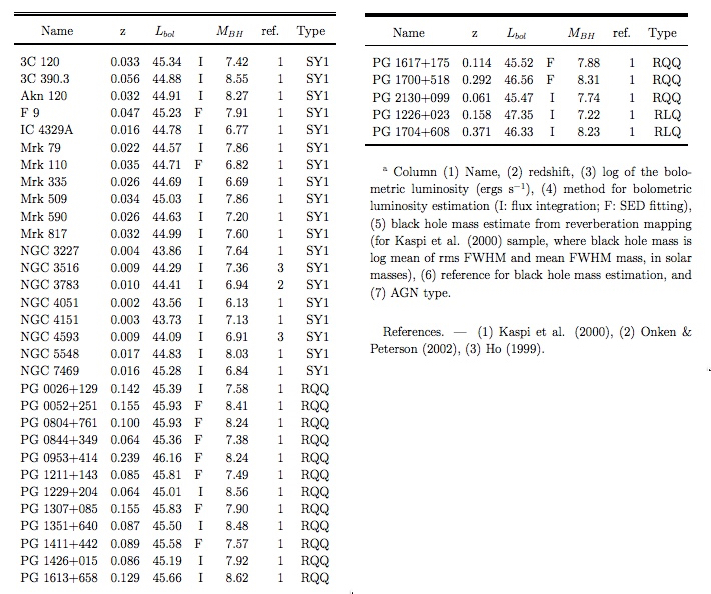
\includegraphics[scale=0.3] {figures/AGNs.jpg}
      \end{figure}
	\end{center}	
	\tiny
	J.-H. Woo, C. M. Urry. \textit{AGN Black Hole Masses and Bolometric Luminosities}. \textit{Astrophys. J.} 579 (2002) 530-544
\end{frame}

\subsection{Eddington Accretion Rate}
\begin{frame}{ Accretion Rate}
	The luminosity is just a fraction of the relativistic energy of the accreting mass, $E=m c^2$. The other fraction goes into the BH making it grow.
	\pause
	\[ L \propto \frac{dE}{dt} = \frac{dm}{dt} c^2 = \frac{dM}{dt} c^2 \]
	\pause
	\[L = \eta \dot{M} c^2\]
	\pause
	$\eta$: Efficiency of the process
\end{frame}


\begin{frame}{ Accretion Rate}
	Accretion produces radiation by conversion of gravitational potential.
	\[ U = \frac{GMm}{r}\]
	\pause
	\[ L \sim \frac{dU}{dt} = \frac{GM}{r} \frac{dm}{dt} = \frac{GM}{r} \dot{M} \]
	\pause
	\[\eta = \frac{GM}{rc^2}	\]	
\end{frame}

\begin{frame}{ Accretion Rate}
	In order to estimate the efficiency, consider the ISCO for Schwarzchild, 
	\[r_{ISCO} = 3r_S = \frac{6GM}{c^2}\]
	\pause
	A particle falling from this orbit into the BH  looses the energy
	\pause
	Hence
	\pause
	\[\eta \sim 0.1 - 0.2 \]	
\end{frame}

\begin{frame}{ Accretion Rate}
	In some books consider the accretion of particles falling from $r=5r_S$, because it gives most of the optical/UV continuum radiation.\\
	\pause
	
	Using this point, one obtains an efficiency of $\eta \sim 0.1$
\end{frame}

\begin{frame}{ Accretion Rate}
	For a typical AGN, $L \sim 10^{47} \textrm{ erg} \cdot \textrm{s}^{-1}$.\\
	\pause
	\begin{itemize}
	\item If $\eta \sim 0.007$ as in the Hydrogen burning process (Nuclear fusion), it gives
	\pause
	\[\dot{M} = \frac{L}{\eta c^2} \sim 250 M_{\odot\ } \cdot \textrm{yr}^{-1} \]
	\pause
	\item If $\eta \sim 0.1 $ we obtain a more realistic value of
	\pause
	\[\dot{M} = \frac{L}{\eta c^2} \sim 250 M_{\odot\ } \cdot \textrm{yr}^{-1} \]
	\pause
	\end{itemize}		
\end{frame}

\begin{frame}{ Accretion Rate}
	\[ \dot{M} = \frac{L}{\eta c^2} = 1.11 \times 10^{23} \frac{L_{44}}{\eta} \left[ \frac{\textrm{gr}}{\textrm{s}}\right]\]	
	\pause
	\[ \dot{M} = 1.77 \times 10^{-2} L_{44} \left ( \frac{\eta}{0.1}\right)^{-1} \left[ \frac{M_{\odot\ }}{\textrm{yr}}\right]\]
\end{frame}

\begin{frame}{Eddington Accretion Rate}
	\[ \dot{M}_E = \frac{L_E}{\eta c^2} =  \frac{4 \pi GM m_p}{\sigma_e \eta c} \]	
	\pause
	\[ \dot{M}_E = 2.67 \times 10^{-8} \left ( \frac{\eta}{0.1}\right)^{-1} \frac{M}{M_{\odot\ } }  \left[ \frac{M_{\odot\ }}{\textrm{yr}}\right]\]
	\pause
	\[ \dot{M}_E = 3 \left ( \frac{\eta}{0.1}\right)^{-1} M_8   \left[ \frac{M_{\odot\ }}{\textrm{yr}}\right]\]
	\pause
	$\dot{M}_E$: Maximum possible accretion rate for a mass $M_8 = \frac{M}{10^8 M_{\odot\ }}$.
\end{frame}

\begin{frame}{Eddington Accretion Rate}
	May $\dot{M} > \dot{M}_E$ ?
	\pause
	\begin{enumerate}
		\item It depends on a careful determination of $\eta$. E.g. if $\eta < 0.1$, the outwards flux is diminished.
		\pause
		\item $\dot{M}_E$ can be exceeded with non-spherical models.
	\end{enumerate}
\end{frame}

\subsection{Growth Time}
\begin{frame}{Growth Time}
	\[ \dot{M} = \frac{dM}{dt} = \frac{L}{\eta c^2} \]
	\pause
	\[ \dot{M} = \frac{dM}{dt} = \frac{L}{L_E} \frac{4 \pi GM m_p}{\sigma_e \eta c} \]
	\pause
	\[ \int \frac{dM}{M} = \frac{L}{L_E} \frac{4 \pi G m_p}{\sigma_e \eta c} \int dt \]
	\pause
	\[ M(t) = M_0 \exp \left( \frac{t}{t_{growth} }\right) \]
	\pause
	\[ t_{growth} = \frac{\sigma_e \eta c}{4 \pi G m_p} \left( \frac{L_E}{L} \right) \]
\end{frame}

\begin{frame}{Growth Time}
	\[ t_{growth} = \frac{\sigma_e \eta c}{4 \pi G m_p} \left( \frac{L_E}{L} \right) \]
	\pause
	\[ t_{growth} = 3.7 \times 10^8 \eta \left( \frac{L_E}{L} \right) [\textrm{yr}]\]
	\pause
	\footnotesize
	For $L \sim L_E$, the BH grows exponentially on time scales of the order $\sim 10^8 \textrm{ yr}$.
\end{frame}

\subsection{Temperatures}
\begin{frame}{Radiation Temperature}
	The \textit{continuum spectrum} of the emitted radiation is characterized by a temperature
	\[ T_{rad} = \frac{h\bar{\nu}}{k_B}\]
	\pause	
	$\bar{\nu}$: frequency of a typical (average) photon
\end{frame}

\begin{frame}{Black Body Temperature}
	For a source with accretion luminosity $L$ and radius $r$, it is defined the \textit{blackbody temperature} through
	\[F= \sigma T_{eff}^4 \]
	\pause	
	$\sigma = 5.6 \times 10^{-5} \frac{\textrm{erg}}{\textrm{cm}^2 \cdot \textrm{s} \cdot \textrm{K}^4 \cdot \textrm{sr}}$\\
	Steffan-Boltzman Constant
	\pause
	\[ T_{eff} = \left( \frac{L}{4\pi r^2 \sigma} \right)^{1/4} \]
\end{frame}

\begin{frame}{Black Body Temperature}	
	Using $L = \frac{GM}{r} \dot{M}$,
	\pause	
	\[ T_{eff} = \left( \frac{GM\dot{M}}{4\pi r^3 \sigma} \right)^{1/4} \]
	\pause
	\[T_{eff} = 1.01 \times 10^6 M_8^{-1/4} \left( \frac{\dot{M}}{\dot{M}_E} \right)^{1/4} \left( \frac{r}{r_S} \right)^{-3/4} \]
\end{frame}

\subsection{Compactness}
\begin{frame}{compactness}	
	One way to estimate the compactness of a source is using the luminosity and the effective surface temperature.
	\[r_{BB} = \sqrt{\frac{L}{4\pi \sigma T_{eff} ^4}}  \]
\end{frame}


\begin{frame}{Example}	
	Consider a system in our galaxy with $L=10^{37} \textrm{ erg} \cdot \textrm{s}^{-1}$
	\pause
	\bigskip
	From the Eddington limit, the mass of the central object must be
	\[ M \geq \frac{L}{1.26 \times 10^{38}} M_{\odot\ } \sim \frac{10^{37}}{10^{38}} M_{\odot\ }  \sim 0.1 M_{\odot\ } \]
\end{frame}

\begin{frame}{Example}	
	If the radiation is in the optical-UV,\\
	\onslide<2->
	
	$\nu_{max} \sim 10^{15} \textrm{Hz}$
	\onslide<3->
	\[ T_{eff} \sim T_c = \frac{10^{15}}{5.88 \times 10^{10}} \sim 10^5 \textrm{K} \]
	\onslide<4->
	\[ r_{bb} \sim 10^{12} \textrm{cm} \sim 10^{7} \textrm{km}\]
	\onslide<5->
	Typical size of a Star!
	
	\onslide<1->
	\tiny
	https://rechneronline.de/spectrum
\end{frame}

\begin{frame}{Example}	
	If the radiation is in soft X-rays at $1 \textrm{ keV}$,\\
	\onslide<2->
	
	$\nu_{max} \sim 10^{17} \textrm{Hz}$
	\onslide<3->
	\[ T_{eff} \sim T_c = \frac{10^{17}}{5.88 \times 10^{10}} \sim 10^7 \textrm{K} \]
	\onslide<4->
	\[ r_{bb} \sim 10^{6} \textrm{cm} \sim 10 \textrm{km}\]
	\onslide<5->
	Typical size of a neutron star or a BH!
	\onslide<1->
	\tiny
	https://rechneronline.de/spectrum
\end{frame}

\begin{frame}{Virial Temperature}	
	$T_{th}$: Temperature reached by the accreted material if all the gravitational energy is transformed into thermal energy.\\
	\pause
	$2\left\langle K \right\rangle + \left\langle U \right\rangle = 0$: Virial Theorem
	\pause
	\[ \left\langle U \right\rangle = \frac{GM(m_p + m_e)}{r}\sim \frac{GMm_p}{r} \]
	\pause
	\[ 2\left\langle K \right\rangle \sim 2 \times \frac{3}{2} k_B T_{th} \]
	\pause
	\[ T_{th} = \frac{GMm_p}{3k_B r} = T_{vir}\]
\end{frame}

\begin{frame}{Temperatures}	
	If the accretion energy is converted directly into radiation escaping without interaction,
	\pause
	\[ T_{rad} \sim T_{th}\]
	\pause
	If the accretion flow is optically thick, the radiation reaches thermal equilibrium with the accreted material before escaping out to the observer,
	\pause
	\[ T_{rad} \sim T_{eff}\]
	\pause
	\bigskip
	In general,
	\pause
	\[ T_{eff} \lesssim T_{rad} \lesssim T_{th}\]
	
\end{frame}






\section{Geodesics in Kerr Spacetime}    
\begin{darkframes}

\subsection{Hamilton-Jacobi Formulation}
\begin{frame}
\Huge
Hamilton-Jacobi Formulation
\end{frame}

\begin{frame}{Hamilton-Jacobi Formulation}
    \[ \mathcal{L} = \frac{1}{2}  g_{\mu\nu} \dot{x}^\mu \dot{x}^\nu \]
    \pause
    \[ p_\mu = \frac{\partial \mathcal{L}}{\partial \dot{x}^\mu} =  g_{\mu\nu} \dot{x}^\nu \]
    \pause
    \[ \mathcal{H} = \frac{1}{2}  g^{\mu\nu} p_\mu p_\nu \]
\end{frame}

\begin{frame}{Hamilton-Jacobi Formulation}
    Hamilton's principal function
    \[ S = S \left( x^\mu ; \lambda \right)\]
    \pause
    \[ p_\mu = \frac{\partial S}{\partial x^\mu} \]
    \pause
    Hamilton-Jacobi Equation
    \pause
    \[  \frac{1}{2}  g^{\mu\nu} \frac{\partial S}{\partial x^\mu} \frac{\partial S}{\partial x^\nu} - \frac{\partial S}{\partial \lambda} =0 \]
\end{frame}

\begin{frame}{Kerr's Solution}
    	Boyer-Lindquist coordinates: $\left(t,r,\theta,\varphi\right)$
     	\begin{align*}
            ds^{2} &= -\frac{\Delta-a^{2}\sin^{2}\theta}{\varrho}dt^{2}-\left(\frac{r^{2}+a^{2}-\Delta}{\varrho}\right)2a\sin^{2}\theta dtd\varphi\nonumber \\
             & +\frac{\varrho}{\Delta}dr^{2}+\varrho d\theta^{2}+\left(\frac{\left(r^{2}+a^{2}\right)^{2}-\Delta a^{2}\sin^{2}\theta}{\varrho}\right)\sin^{2}\theta d\varphi^{2}.
      	\end{align*}
     	\pause
   	$$\varrho  = r^{2}+a^{2}\cos^{2}\theta$$
    $$\Delta =  r^{2}-2Mr+a^{2}$$
\end{frame}

\begin{frame}{Kerr's Solution}
     	\begin{align*}
            \left( \frac{\partial}{\partial s} \right)^{2} = &- \frac{A}{\varrho \Delta} \left( \frac{\partial}{\partial t} \right)^{2} - \frac{4aMr}{\varrho \Delta} \left( \frac{\partial}{\partial t} \right) \left( \frac{\partial}{\partial \varphi} \right) +\frac{\Delta}{\varrho}\left( \frac{\partial}{\partial r} \right)^2 \nonumber \\
             & + \frac{1}{\varrho} \left( \frac{\partial}{\partial \theta} \right)^{2} + \frac{\Delta - a^2 \sin^2 \theta}{\varrho \Delta \sin^{2}\theta} \left( \frac{\partial}{\partial \varphi} \right)^{2}
      	\end{align*}
    \pause
    $$A = (r^2 + a^2)^2 -a^2 \Delta \sin^2 \theta$$ 	
   	$$\varrho  = r^{2}+a^{2}\cos^{2}\theta$$
    $$\Delta =  r^{2}-2Mr+a^{2}$$
\end{frame}

\begin{frame}{Hamilton-Jacobi Formulation}
    Hamilton-Jacobi Equation
     \[ 2 \frac{\partial S}{\partial \lambda}  = g^{\mu\nu} \frac{\partial S}{\partial x^\mu} \frac{\partial S}{\partial x^\nu} \]
    \pause
    \begin{align*}
           2 \frac{\partial S}{\partial \lambda} = &- \frac{A}{\varrho \Delta} \left( \frac{\partial S}{\partial t} \right)^2 - \frac{4aMr}{\varrho \Delta} \left( \frac{\partial S}{\partial t} \right) \left( \frac{\partial S}{\partial \varphi} \right) +\frac{\Delta}{\varrho}\left( \frac{\partial S}{\partial r} \right)^2 \nonumber \\
             & + \frac{1}{\varrho} \left( \frac{\partial S}{\partial \theta} \right)^{2} + \frac{\Delta - a^2 \sin^2 \theta}{\varrho \Delta \sin^{2}\theta} \left( \frac{\partial S}{\partial \varphi} \right)^{2}
    \end{align*}   
\end{frame}

\begin{frame}{Hamilton-Jacobi Formulation}
    Hamilton Principal Function
    \[S = \frac{1}{2} \lambda \delta -\varepsilon t +\ell_z \varphi + S_r (\theta) + S_\theta (\theta)\]
	Separation of the Hamilton-Jacobi Equation. Carter Constant
	\begin{align*}
	&\Delta \left( \frac{dS_r}{dr}\right)^2 - \frac{1}{\Delta} \left[ (r^2 +a^2) \varepsilon - a \ell_z \right]^2 + (\ell_z - a \varepsilon)^2 + \delta r^2  =\\
	& -\left( \frac{dS_\theta}{d\theta}\right)^2 - \left(\frac{\ell_z^2}{\sin^2 \theta} - a^2 \varepsilon^2 + \delta a^2 \right)\cos^2 \theta = \mathcal{C}
	\end{align*}      
\end{frame}

\begin{frame}{Hamilton-Jacobi Formulation}
	Separation of the Hamilton-Jacobi Equation. Carter Constant
	\begin{align*}
	\Delta \left( \frac{dS_r}{dr}\right)^2 &= \frac{1}{\Delta} \left[ (r^2 +a^2) \varepsilon - a \ell_z \right]^2 - \left[ \mathcal{C} + (\ell_z - a \varepsilon)^2 + \delta r^2 \right]\\ 
	\left( \frac{dS_\theta}{d\theta}\right)^2 &= \mathcal{C} - \left( \frac{\ell_z^2}{\sin^2 \theta} - a^2 \varepsilon^2 + \delta a^2 \right) \cos^2 \theta	
	\end{align*}      
\end{frame}

\begin{frame}{Hamilton-Jacobi Formulation}
	\begin{align*}
	S_r &= \int \frac{\sqrt{R(r')}}{\Delta}dr'\\
	S_\theta &= \int \sqrt{\Theta(\theta')}d\theta'
	\end{align*}
	\pause 
	\begin{align*}
	R(r) &= \left[ (r^2 +a^2) \varepsilon - a \ell_z \right]^2 - \Delta \left[\mathcal{C} + (\ell_z - a \varepsilon)^2 + \delta r^2 \right]\\
	\Theta(\theta) &= \mathcal{C} - \left[ \frac{\ell_z^2}{\sin^2 \theta} + a^2 \left(\delta - \varepsilon^2 \right) \right] \cos^2 \theta
	\end{align*}      
\end{frame}

\begin{frame}{Carter Constant}
	\[\left( \frac{dS_\theta}{d\theta}\right)^2 = \mathcal{C} - \left( \frac{\ell_z^2}{\sin^2 \theta} - a^2 \varepsilon^2 + \delta a^2 \right) \cos^2 \theta\] 
	\bigskip
	\pause
	
	\[ \mathcal{C} = p_\theta^2 + p_\varphi^2 \cot^2 \theta + a^2 (\delta - \varepsilon^2) \cos^2 \theta \]     
\end{frame}

\begin{frame}{Carter Constant}
	Schwarzschild:		
	\[ \mathcal{C} = \left( p_\theta^2 + \frac{p_\varphi^2}{\sin^2 \theta} \right) - p_\varphi^2 = \ell^2 - \ell_z^2 \]   
	where $\ell = p_\theta^2 + \frac{p_\varphi^2}{\sin^2 \theta}$ is the total angular momentum.
\end{frame}

\begin{frame}{Carter Constant}
	Kerr:
	\pause		
	\begin{itemize}
	\item $\mathcal{C}$ has not a direct physical interpretation.
	\item $\mathcal{C}=0$ implies that the motion is in the equatorial plane.
	\end{itemize}
\end{frame}



\subsection{Equations of Motion}
\begin{frame}
	\huge
    {Equations of Motion}
\end{frame}

\begin{frame}{Equations of Motion}
    Hamilton Canonical Equations
    \pause
    \[ \dot{x}^\mu = p^\mu = g^{\mu \nu} p_\nu = g^{\mu\nu} \frac{\partial S}{ x^\nu} \]
\end{frame}

\begin{frame}{Equations of Motion}
    \footnotesize

    \begin{align*}
    \varrho^2 \dot{r}^2 &= R \\
    \varrho^2 \dot{\theta}^2 &= \Theta \\
    \varrho \dot{\varphi} &= \frac{1}{\Delta} \left[ 2aMr\varepsilon + (\varrho - 2Mr)\frac{\ell_z}{\sin^2 \theta} \right] \\
    \varrho \dot{t} &= \frac{1}{\Delta} \left[ A\varepsilon + 2aMr \ell_z \right]
    \end{align*}
    \pause
    \begin{align*}
    R(r) &= \left[ (r^2 +a^2) \varepsilon - a \ell_z \right]^2 - \Delta \left[\mathcal{C} + (\ell_z - a \varepsilon)^2 + \delta r^2 \right]\\
	\Theta(\theta) &= \mathcal{C} - \left[ \frac{\ell_z^2}{\sin^2 \theta} + a^2 \left(\delta - \varepsilon^2 \right) \right] \cos^2 \theta\\
    A &= (r^2 + a^2)^2 - a^2 \Delta \sin^2 \theta \\
    \varrho  &= r^{2}+a^{2}\cos^{2}\theta \\
    \Delta &= r^{2}-2Mr+a^{2} 
    \end{align*}
\end{frame}

\subsection{Imaging a Black Hole}
\begin{frame}
	\huge
    {Imaging a Black Hole}
\end{frame}

\begin{frame}
	\huge
    {Image Plane of a Distant Observer}
\end{frame}

\begin{frame}{Image Plane of a Distant Observer}
    \begin{itemize}
    \item A distant observer receives the electromagnetic radiation from the accretion disk, around the black hole.
    \pause
    \item It is usual to define a plane of observation and consider the photons with momentum orthogonal to the plane. These photons' trajectories are integrated backwards in time to find the position of the emission point in the disk.
    \end{itemize}
\end{frame}

\end{darkframes}
\begin{frame}{Image Plane of a Distant Observer}
	\begin{center}
      \begin{figure}
      	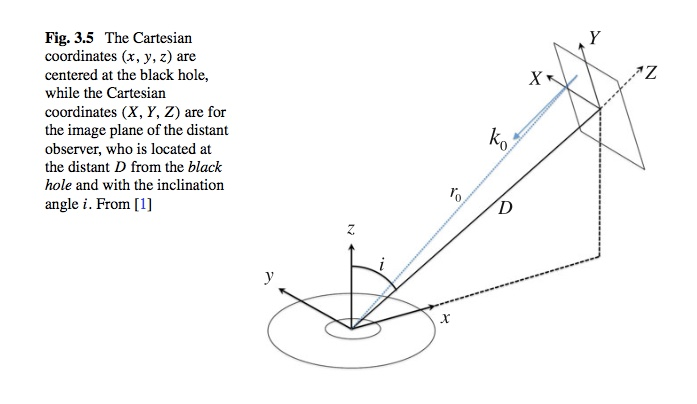
\includegraphics[scale=0.35] {figures/diskobservation.jpeg}
      \end{figure}
	\end{center}	
\end{frame}

\begin{darkframes}

\begin{frame}{Coordinate Systems}
    \begin{itemize}
    \item $(X,Y,Z)$: Cartesian coordinates in the image plane
    \pause
    \item $(x,y,z)$: Cartesian coordinates centered at the black hole.
    \pause
    \item $i$: Inclination angle of the observer with respect to the $z$ direction.
    \pause
    \item $D$: Distance observer-black hole.
    \end{itemize}
\end{frame}

\begin{frame}{Coordinate transformations}
	\begin{align*}
    x &= D\sin i - Y \cos i + Z\sin i\\
    y &= X\\
    z &= D\cos i + Y \sin i + Z\cos i
    \end{align*}
    
    \begin{align*}
    r &= \sqrt{x^2 + y^2 + z^2}\\
    \theta &= \arccos \left( \frac{z}{r} \right)\\
    \varphi &= \arctan \left( \frac{z}{r} \right)
    \end{align*}
\end{frame}

\begin{frame}
	\huge
    {Photon Trajectory Tracing}
\end{frame}

\begin{frame}{Photon Trajectory Tracing}
	Consider a photon received at $(X_0,Y_0,0)$ with 3-momentum $\textbf{k}_0 = -k_0 \hat{Z}$, i.e. perpendicular to the observer plane.\\
	
	The initial conditions for the position of the photon (to trace back the trajectory), as seen from the black hole and in spherical coordinates, are
    \begin{align*}
	t_0 &= 0\\     
    r_0 &= \sqrt{X_0^2 + Y_0^2 + D^2}\\
    \theta_0 &= \arccos \left( \frac{Y_0 \sin i + D \cos i}{r_0} \right)\\
    \varphi_0 &= \arctan \left( \frac{X_0}{D \sin i - Y_0 \cos i} \right)
    \end{align*}
\end{frame}

\begin{frame}{Photon Trajectory Tracing}
	The initial conditions for the 4-momentum of the photon $k^\mu$ (to trace back the trajectory), as seen from the black hole and in spherical coordinates, are calculated with the transformation law,
	\[ k^\mu = \frac{\partial x^\mu}{\partial \bar{x}^\alpha} \bar{k}^\alpha \]
	\pause
	\footnotesize
    \begin{align*}
	k_0^r &= -\frac{D}{r} k_0\\     
    k_0^\theta &= \frac{\cos i - (Y_0 \sin i + D \cos i)\frac{D}{r_0^2} }{\sqrt{X_0^2 + (D \sin i - Y_0 \cos i)^2}} k_0\\
    k_0^\varphi &= \frac{X_0 \sin i}{X_0^2 + (D \sin i - Y_0 \cos i)^2} k_0
    \end{align*}
\end{frame}

\begin{frame}{Photon Trajectory Tracing}
	The $k^t_0$ component of the initial 4-momentum is calculated by the condition $g_{\mu\nu} g^\mu k`^\nu = 0 $,
	\[ k_0 ^t = \sqrt{(k_0^r)^2 + r_0^2 (k_0^\theta)^2 + r_0^2 \sin^2 \theta_0 (k_0^\varphi)^2}\]
\end{frame}

\begin{frame}{Photon Trajectory Tracing}
	Given the initial conditions for position and momentum, it is possible to trace  the trajectory of any photon in the observer plane back to the accretion disk.
\end{frame}

\begin{frame}
	\huge
    {Non-Coordinate Basis}
\end{frame}

\begin{frame}{Tetrads}
	Introduce a non-coordinate basis or orthonormal tetrad,
	\pause
	\begin{align*}
	\textbf{E}_{(a)} &= E_{(a)}^\mu \partial_\mu \\
	\textbf{E}^{(a)} &= E^{(a)}_\mu dx^\mu,
	\end{align*}
	subject to the conditions
	\begin{align*}
	\eta_{(a)(b)} &= E_{(a)}^\mu E_{(b)}^\nu g_{\mu\nu} \\
	\eta^{(a)(b)} &= E^{(a)}_\mu E^{(b)}_\nu g{\mu\nu}
	\end{align*}
	and $ det |E_{(a)^\mu} | >0$ (to preserve the orientation).
\end{frame}

\begin{frame}{Tetrads}
	Components of a vector in the orthonormal tetrad basis,
	\pause
	\begin{align*}
	V^{(a)} &= E^{(a)}_\mu V^\mu \\
	V_{(a)} &= E_{(a)}^\mu V_\mu
	\end{align*}
\end{frame}

\begin{frame}{General Metric}
	Consider a general stationary, axisymmetric, asymptotically flat metric
	\[ ds^2 = -e^{2\alpha(r)}dt^2 + e^{2\beta(r)} dr^2 + e^{2\gamma(r,\theta)} d\theta^2 + e^{2\epsilon(r,\theta)} (d\varphi-\omega dt)^2\] 
	\pause
	We identify the \textit{locally non-rotating observers} as those whose world-lines have 
	\pause
	\begin{align*}
	r &= \textrm{constant} \\
	\theta &= \textrm{constant}\\
	\varphi &= \omega t+\textrm{constant}
	\end{align*}
\end{frame}

\begin{frame}{General Metric}
	The non-coordinate basis of the locally non-rotating observers is given by the tetrad
	\begin{align*}
	E^\mu _{(t)} &= \left( e^{-\beta}, 0, 0, \omega e^{-\beta} \right)\\
	E^\mu _{(r)} &= \left( 0, e^{-\alpha}, 0, 0 \right)\\
	E^\mu _{(\theta )} &= \left( 0, 0, e^{-\gamma}, 0 \right)\\
	E^\mu _{(\varphi )} &= \left( 0, 0, 0, e^{-\epsilon} \right)
	\end{align*}
\end{frame}

\begin{frame}{General Metric}
	and the dual basis,	
	\begin{align*}
	E_\mu ^{(t)} &= \left( e^{\beta}, 0, 0, 0 \right)\\
	E_\mu ^{(r)} &= \left( 0, e^{\alpha}, 0, 0 \right)\\
	E_\mu ^{(\theta )} &= \left( 0, 0, e^{\gamma}, 0 \right)\\
	E_\mu ^{(\varphi )} &= \left( -\omega e^{\epsilon}, 0, 0, e^{\epsilon} \right)
	\end{align*}
\end{frame}

\begin{frame}{Kerr Metric}
	For the particular case of the Kerr metric the tetrad describing 	the non-coordinate basis of the locally non-rotating observers is
	\begin{align*}
	E^\mu _{(t)} &= \left( \sqrt{\frac{A}{\varrho \Delta}}, 0, 0, \frac{2Mar}{\sqrt{A \varrho \Delta}} \right)\\
	E^\mu _{(r)} &= \left( 0, \sqrt{\frac{\Delta}{\varrho}}, 0, 0 \right)\\
	E^\mu _{(\theta )} &= \left( 0, 0, \frac{1}{\sqrt{\varrho}}, 0 \right)\\
	E^\mu _{(\varphi )} &= \left( 0, 0, 0, \frac{1}{\sin \theta}\sqrt{\frac{\varrho}{A}} \right)
	\end{align*}
\end{frame}

\begin{frame}{Kerr Metric}
	and the dual basis is
	\begin{align*}
	E_\mu ^{(t)} &= \left( \sqrt{\frac{\varrho \Delta}{A}}, 0, 0, 0 \right)\\
	E_\mu ^{(r)} &= \left( 0, \sqrt{\frac{\varrho}{\Delta}}, 0, 0 \right)\\
	E_\mu ^{(\theta )} &= \left( 0, 0, \sqrt{\varrho}, 0 \right)\\
	E_\mu ^{(\varphi )} &= \left( -\frac{2Mar \sin \theta}{\sqrt{\varrho A}}, 0, 0, \sqrt{\frac{A}{\varrho}} \sin \theta \right)
	\end{align*}
\end{frame}

\begin{frame}{Momentum Components in the Non-Coordinate Basis}
	The momentum components of a particle moving in Kerr's spacetime are
	\[ p_\mu = \frac{\partial S}{\partial x^\mu} \]
	\pause
	\begin{align*}
	p_t &= -\varepsilon\\
	p_r &= \frac{\sqrt{R}}{\Delta}\\
	p_\theta &= \sqrt{\Theta}\\
	p_\varphi &= \ell_z
	\end{align*}
\end{frame}

\begin{frame}{Momentum Components in the Non-Coordinate Basis}
	In the non-coordinate basis, the momentum components of a particle are
	\[ p^{(a)} = E^{(a)}_\mu p^\mu = \eta ^{(a)(b)} E_{(b)}^\mu p_\mu  \]
	\pause
	\begin{align*}
	p^(t) &= -E_{(t)}^\mu p_\mu\\
	p^r &= E_{(r)}^\mu p_\mu\\
	p^\theta &= E_{(\theta)}^\mu p_\mu\\
	p^\varphi &= E_{(\varphi)}^\mu p_\mu
	\end{align*}
\end{frame}

\begin{frame}
	\huge
    {Celestial Coordinates}
\end{frame}

\begin{frame}{Celestial Coordinates}
	The position of a photon in the image plane of the distant observer is given by the coordinates 
	\[\begin{cases}
	X_0 &= \alpha = \lim_{r\rightarrow\infty} \left( \frac{rp^{(\varphi)}}{p^{(t)}} \right) \\
	Y_0 &= \beta = \lim_{r\rightarrow\infty} \left( \frac{rp^{(\theta)}}{p^{(t)}} \right)
	\end{cases}\]
\end{frame}

\begin{frame}{Celestial Coordinates}
	\[\begin{cases}
	\alpha &= -\xi \csc i\\	
	\beta &= \pm \sqrt{\eta + a^2 \cos^2 i - \xi^2 \cot^2 i}
	\end{cases}\]
	\pause
	\[\begin{cases}
    \xi &= \frac{\ell_z}{\varepsilon}\\
    \eta &= \frac{\mathcal{C}}{\varepsilon^2}
	\end{cases}\]
\end{frame}


\begin{frame}
	\huge
    {Black Hole's Shadow}
\end{frame}

\begin{frame}{Effective Potential for Photons}
    \begin{align*}
    R(r) &= \left[ (r^2 +a^2) \varepsilon - a \ell_z \right]^2 - \Delta \left[\mathcal{C} + (\ell_z - a \varepsilon)^2 + \delta r^2 \right]\\
	\Theta(\theta) &= \mathcal{C} - \left[ \frac{\ell_z^2}{\sin^2 \theta} + a^2 \left(\delta - \varepsilon^2 \right) \right] \cos^2 \theta
    \end{align*}
    \pause
    Consider these expressions for photons, $\delta=0$, and using the quantities
    \[\begin{cases}
    \xi &= \frac{\ell_z}{\varepsilon}\\
    \eta &= \frac{\mathcal{C}}{\varepsilon^2}
	\end{cases}\]    
\end{frame}

\begin{frame}{Effective Potential for Photons}
    \begin{align*}
    R(r) &= \left[ r^2 +a^2  - a \xi  \right]^2 \varepsilon^2- \Delta \left[\eta + (\xi - a )^2 \right]\varepsilon^2\\
	\Theta(\theta) &= \eta \varepsilon^2   - \left[ \frac{\xi^2}{\sin^2 \theta} - a^2 \right] \varepsilon^2 \cos^2 \theta
    \end{align*}
  
\end{frame}

\begin{frame}{Effective Potential for Photons}
	\begin{align*}
	\mathcal{R}(r) &= \frac{R(r)}{\varepsilon^2} = \left[ r^2 +a^2  - a \xi  \right]^2 - \Delta \left[\eta + (\xi - a )^2 \right] \\
	\vartheta (\theta) &= \frac{\Theta(\theta)}{\varepsilon^2} = \left[\eta + (\xi - a )^2 \right] - \left[ a \sin \theta - \xi \csc \theta \right]^2
	\end{align*} 
	\pause 
	\[\Delta = r^{2}-2Mr+a^{2} \] 
\end{frame}

\begin{frame}{Equations of Motion for Photons}
	\begin{align*}
    \varrho^2 \dot{r}^2 &= \mathcal{R} \\
    \varrho^2 \dot{\theta}^2 &= \vartheta \\
    \varrho \dot{\varphi} &= \frac{1}{\Delta} \left[ 2aMr + \frac{\xi (\varrho - 2Mr)}{\sin^2 \theta} \right] \\
    \varrho \dot{t} &= \frac{1}{\Delta} \left[ A + 2aMr \xi \right]
    \end{align*}
\end{frame}

\begin{frame}{Photon Sphere}
	Circular motion of photons: $\dot{r} = 0$
	\pause
	\[\begin{cases}
	\mathcal{R} &= 0\\
	\partial_r \mathcal{R} &= 0
	\end{cases}\]
\end{frame}

\begin{frame}{Photon Sphere}
	Solving for $\xi$ and $\eta$ we obtain these quantities for the circular orbit as functions of the parameter $r$,
	\pause
	\begin{align*}
	\xi_{c} &= \frac{M(r^2 -a^2) - r \Delta}{a(r-M)} \\
	\eta_{c} &= \frac{r^3 \left[ 4M\Delta - r (r-M)^2\right]}{a^2(r-M)^2}
	\end{align*}
\end{frame}

\begin{frame}{Photon Sphere}
	There are three possible cases regarding the stability of circular orbits of photons
	\pause
	\begin{enumerate}
	\item If $\partial_r^2 \mathcal{R} > 0$ : Stable circular orbits
	\pause
	\item If $\partial_r^2 \mathcal{R} < 0$ : Unstable circular orbits. The photon straddles the boundary between two regions: $\partial_r \mathcal{R} = 0$; if perturbed one way it falls into the horizon, if perturbed the other way it flies outwards.
	\pause
	\item If $\partial_r^2 \mathcal{R} = 0$ : Marginally stable circular orbit (Photon Sphere). $r=r_{ps}$.
	\end{enumerate}	 
\end{frame}

\begin{frame}{Black Hole's Shadow}
	\begin{align*}
	\alpha &= -\xi_c \csc i\\	
	\beta &= \sqrt{\eta_c + a^2 \cos^2 i - \xi_c^2 \cot^2 i}
	\end{align*}
	\pause
	\begin{align*}
	\xi_c &= \frac{M(r^2 -a^2) - r \Delta}{a(r-M)} \\
	\eta_c &= \frac{r^3 \left[ 4M\Delta - r (r-M)^2\right]}{a^2(r-M)^2}
	\end{align*}
\end{frame}

\begin{frame}{Black Hole's Shadow}
	Schwarzschild's Black Hole:	
	\[ \alpha^2 + \beta^2 = R_{shadow}^2\]
	\pause
	\[ R_{shadow} = \sqrt{27 M^2} \]
\end{frame}

\begin{frame}{Shadow of Sagittarius A*}
	$M_{SgrA*} = 4 \times 10^6 M_\odot\ $\\
	\bigskip
	\pause
	$r_H = 2 M = \frac{2GM}{c^2}$\\
	\pause
	$r_H = 1.2 \times 10^{10} \textrm{ m.} = 1.2 \times 10^{7} \textrm{ km.}$ \\
	\pause
	$r_H = 0.1 \textrm{ AU} $\\
	\bigskip
	\pause
	$R_{shadow} = \sqrt{27 M^2} = 3 \sqrt{3} M$\\
	\pause
	$R_{shadow} = 3 \sqrt{3} \frac{GM}{c^2} = 3 \times 10^{10} \textrm{ m.}$ \\
	\pause
	$R_{shadow} = 3 \times 10^{7} \textrm{ km.} = 0.2 \textrm{ AU} $ \\
\end{frame}

\begin{frame}{Shadow of Sagittarius A*}
	$R_{shadow} = 0.2 \textrm{ AU} = 9.7 \times 10^{-10} \textrm{ kpc}$ \\
	\bigskip
	\pause
	$D = 8 \textrm{ kpc} $\\
	\bigskip
	$\theta_{shadow} = \frac{R_{shadow}}{D}$\\
	\pause
	$\theta_{shadow} = 1.2 \times 10^{-11} \textrm{ rad}$\\
	\pause
	$\theta_{shadow} = 2.5$ $\mu$arcsec
\end{frame}

\begin{frame}{Shadow of Sagittarius A*}
	Very Long Baseline Interferometry (VLBI)\\
	\bigskip	
	\pause
	$\theta_{res} \sim \frac{\lambda}{d}$\\
	\bigskip
	\pause
	$\lambda \sim 1 \textrm{ mm}$\\
	\pause
	$d \sim 10^3 \textrm{ km}$\\
	\bigskip
	\pause
	$\theta_{res} \sim 10$ $\mu$arcsec	
\end{frame}

\begin{frame}{Next Lecture}
  	\Large
	{08. Accretion}
\end{frame}






\begin{frame}
	\Large
	{Alternative derivation of the Celestial Coordinates}
\end{frame}

\begin{frame}{Celestial Coordinates}
    \begin{itemize}
    \item A distant observer receives the electromagnetic radiation from the surroundings of the black hole.
    \pause
    \item Let the observer be at $r\rightarrow \infty$  with inclination angle $i$ (between the rotation axis of the black hole and the observer's line of sight).
    \pause
    \item The celestial coordinates $(\alpha, \beta )$ are the apparent angular distances of the image on the celestial sphere measured by the observer.
    \end{itemize}
\end{frame}

\begin{frame}{Celestial Coordinates}
	\begin{itemize}
	\item The distant observer may set up a euclidean coordinate system $(x,y,z)$ with the black hole at the origin and its rotation axis along $z$.
	\pause
	\item Using the Boyer-Lindquist coordinates describing the black hole, the observer will be located at some coordinates $(r_0, \theta_0, \varphi_0)$, with  $r_0$ very large.
    	\end{itemize}
\end{frame}

\end{darkframes}

\begin{frame}{Celestial Coordinates}
	\begin{center}
      \begin{figure}
      	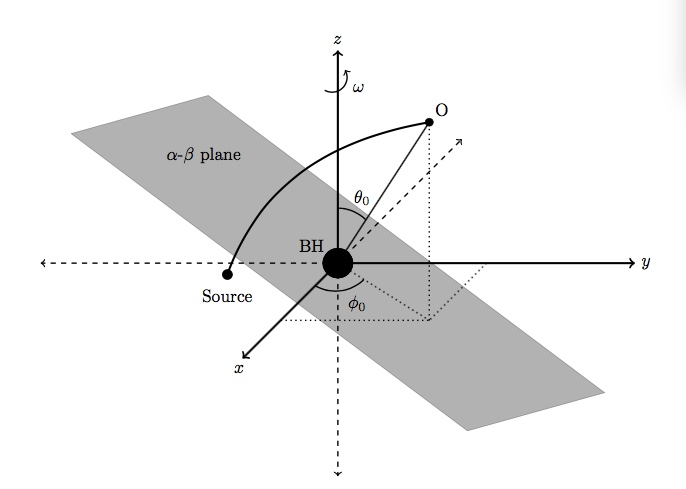
\includegraphics[scale=0.35] {figures/celestialcoordinates1.jpeg}
      \end{figure}
	\end{center}	
\end{frame}

\begin{darkframes}

\begin{frame}{Celestial Coordinates}
	\begin{itemize}
	\item Note that the inclination angle is precisely $\theta_0 = i$. Hence the position of the observer is $(r_0, i, \varphi_0)$
	\pause
	\item Without loosing generality, we rotate the $(x,y,z)$ system so that the angular position of the observer in the Boyer-Lindquist coordinates is $\varphi_0 = 0$. 
	\pause
	\item The position of the observer becomes $(r_0, i, 0)$
	\pause
	\item Then, the observer lies in the $x-z$ plane while the $y$-axis lies in the $(\alpha, \beta)$ plane (remember that the observer plane is perpendicular to the line of sight).  	 
    	\end{itemize}
\end{frame}

\end{darkframes}

\begin{frame}{Celestial Coordinates}
	\begin{center}
      \begin{figure}
      	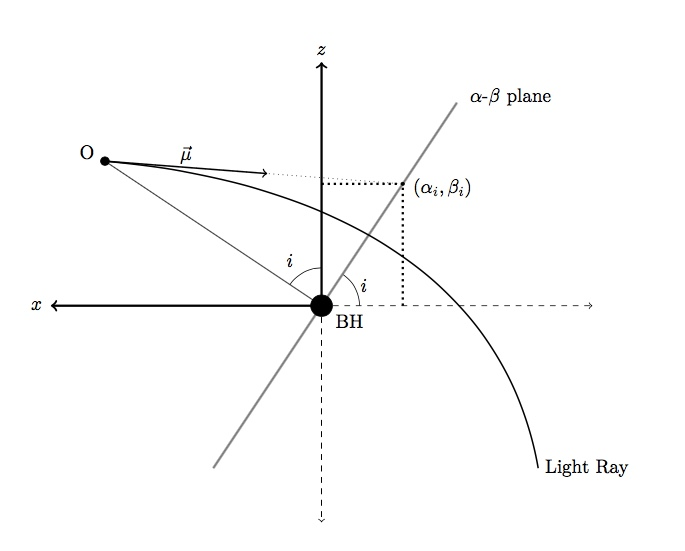
\includegraphics[scale=0.35] {figures/celestialcoordinates2.jpeg}
      \end{figure}
	\end{center}	
\end{frame}

\begin{darkframes}

\begin{frame}{Trajectory of a Light Ray}
	In the observer's reference frame, an incoming light ray trajectory may be decribed by a parametric curve
	\[ \begin{cases}
	X = X(r)\\
	Y = Y(r)\\
	Z = Z(r)\\
	\end{cases} \] 
	such that
	\[ r^2 = X^2 (r) + Y^2 (r) + Z^2 (r) \]	 
\end{frame}	

\begin{frame}{Trajectory of a Light Ray}
	The tangent vector to this parametric curve at the observer's location is
	\[ \vec{\mu} = (\mu_1, \mu_2, \mu_3) = \left( \left. \frac{dX}{dr}\right|_{r_0}, \left. \frac{dY}{dr} \right|_{r_0}, \left. \frac{dZ}{dr} \right|_{r_0} \right) \]	 
\end{frame}
	
\begin{frame}{Trajectory of a Light Ray}
	From the point of view of the observer, this tangent vector defines the trajectory of the photon as a straight line which intersects the observer's celestial plane at the coordinates $(\alpha_i, \beta_i)$ and can be written parametrically as
	\[ \frac{x-x_0}{\mu_1} = \frac{y-y_0}{\mu_2} = \frac{z-z_0}{\mu_3}\]
\end{frame}

\begin{frame}{Trajectory of a Light Ray}
$(x_0, y_0, z_0)$ are the coordinates of the observer's position.\\
\pause
This can be written as
\[ (x_0, y_0, z_0) = (r_0 \sin i, 0, r_0 \cos i)\]	
\pause
The celestial coordinates $(\alpha_i, \beta_i)$ can be written as
\[ (\alpha_i, \beta_i) = (x_i, y_i, z_i) = (-\beta_i \cos i, \alpha_i, \beta_i \sin i)\]
\end{frame}

\begin{frame}{Trajectory of a Light Ray}
	\[ \frac{x-x_0}{\mu_1} = \frac{y-y_0}{\mu_2} = \frac{z-z_0}{\mu_3}\]
	\pause
	\[ \frac{-\beta_i \cos i-r_0 \sin i}{\mu_1} = \frac{\alpha_i}{\mu_2} = \frac{\beta_i \sin i-r_0 \cos i}{\mu_3}\]
\end{frame}

\begin{frame}{Trajectory of a Light Ray}
	Using the transformation between cartesian and spherical coordinates,
	\footnotesize
	\begin{align*}
	X(r) &= r \sin \theta \cos \varphi\\
	Y(r) &= r \sin \theta \sin \varphi\\
	Z(r) &= r \cos \theta,
	\end{align*}
	\normalsize
	we obtain the components of $\vec{\mu}$,
	\footnotesize
	\begin{align*}
	\mu_1 &=  \left. \frac{dX}{dr}\right|_{r_0} = \sin i + r_0 \cos i \left. \frac{d \theta}{dr}\right|_{r_0}\\
	\mu_2 &=  \left. \frac{dY}{dr}\right|_{r_0} = r_0 \sin i \left. \frac{d \varphi}{dr}\right|_{r_0}\\
	\mu_3 &=  \left. \frac{dZ}{dr}\right|_{r_0} = \cos i - r_0 \sin i \left. \frac{d \theta}{dr}\right|_{r_0}
	\end{align*}
\end{frame}

\begin{frame}{Trajectory of a Light Ray}
	\[ \frac{-\beta_i \cos i-r_0 \sin i}{\mu_1} = \frac{\alpha_i}{\mu_2} = \frac{\beta_i \sin i-r_0 \cos i}{\mu_3}\]
	\bigskip
	\pause
	\[ \frac{-\beta_i \cos i-r_0 \sin i}{\sin i + r_0 \cos i \left. \frac{d \theta}{dr}\right|_{r_0}} = \frac{\alpha_i}{r_0 \sin i \left. \frac{d \varphi}{dr}\right|_{r_0}} = \frac{\beta_i \sin i-r_0 \cos i}{\cos i - r_0 \sin i \left. \frac{d \theta}{dr}\right|_{r_0}}\]
\end{frame}

\begin{frame}{Celestial Coordinates}
	\begin{align*}
	\alpha_i &= \lim_{r_0 \rightarrow \infty} -r_0^2 \sin^2 \theta_0 \left. \frac{d\varphi}{dr}\right|_{r_0}\\	
	\beta_i &= \lim_{r_0 \rightarrow \infty} r_0^2 \left. \frac{d\theta}{dr}\right|_{r_0}
	\end{align*}
\end{frame}

\begin{frame}{Celestial Coordinates}
Using the equations of motion for the photons, we obtain
	\begin{align*}
	\alpha_i &= -\xi \csc i\\	
	\beta_i &= \sqrt{\eta + a^2 \cos^2 i - \xi^2 \cot^2 i}
	\end{align*}
\end{frame}

  
  \end{darkframes}
\end{document}
